\documentclass[../main.tex]{subfiles}
\begin{document}
    \subsection {Выборочные коэффициенты корреляции}
    \begin{table}[H]
        \centering
        \begin{tabular}{|c|c|c|c|}
            \hline
            & $r$ & $r_S$ & $r_Q$\\\hline
            $\rho=0$ & & &\\\hline
            $E(z)$ & 0.0066 & -0.0008 & 0.0\\\hline
            $E(z^2)$ & 0.0297 & 0.0276 & 0.04\\\hline
            $D(z)$ & 0.0567 & 0.0581 & 0.0553\\\hline
            \hline
            $\rho=0.5$ & & &\\\hline
            $E(z)$ & 0.5081 & 0.4722 & 0.4\\\hline
            $E(z^2)$ & 0.2582 & 0.223 & 0.16\\\hline
            $D(z)$ & 0.0281 & 0.0327 & 0.047\\\hline
            \hline
            $\rho=0.9$ & & &\\\hline
            $E(z)$ & 0.9026 & 0.8767 & 0.8\\\hline
            $E(z^2)$ & 0.8148 & 0.7686 & 0.64\\\hline
            $D(z)$ & 0.0027 & 0.0046 & 0.0283\\\hline
        \end{tabular}
        \caption{Характеристики распределения размерностью n = 20}
    \end{table}
    
    \begin{table}[H]
        \centering
        \begin{tabular}{|c|c|c|c|}
            \hline
            & $r$ & $r_S$ & $r_Q$\\\hline
            $\rho=0$ & & &\\\hline
            $E(z)$ & 0.0035 & 0.0042 & 0.0\\\hline
            $E(z^2)$ & 0.008 & 0.0078 & 0.0044\\\hline
            $D(z)$ & 0.0181 & 0.0183 & 0.017\\\hline
            \hline
            $\rho=0.5$ & & &\\\hline
            $E(z)$ & 0.5029 & 0.4836 & 0.3333\\\hline
            $E(z^2)$ & 0.2529 & 0.2338 & 0.1111\\\hline
            $D(z)$ & 0.0101 & 0.0114 & 0.0155\\\hline
            \hline
            $\rho=0.9$ & & &\\\hline
            $E(z)$ & 0.9 & 0.8837 & 0.7333\\\hline
            $E(z^2)$ & 0.8101 & 0.7809 & 0.5378\\\hline
            $D(z)$ & 0.0007 & 0.0012 & 0.0092\\\hline
        \end{tabular}
        \caption{Характеристики распределения размерностью n = 60}
    \end{table}
    
    \begin{table}[H]
        \centering
        \begin{tabular}{|c|c|c|c|}
            \hline
            & $r$ & $r_S$ & $r_Q$\\\hline
            $\rho=0$ & & &\\\hline
            $E(z)$ & 0.0019 & 0.0026 & 0.0\\\hline
            $E(z^2)$ & 0.0047 & 0.0048 & 0.0064\\\hline
            $D(z)$ & 0.011 & 0.011 & 0.0104\\\hline
            \hline
            $\rho=0.5$ & & &\\\hline
            $E(z)$ & 0.4987 & 0.4787 & 0.32\\\hline
            $E(z^2)$ & 0.2487 & 0.2291 & 0.1024\\\hline
            $D(z)$ & 0.0058 & 0.0062 & 0.0086\\\hline
            \hline
            $\rho=0.9$ & & &\\\hline
            $E(z)$ & 0.8998 & 0.887 & 0.72\\\hline
            $E(z^2)$ & 0.8097 & 0.7867 & 0.5184\\\hline
            $D(z)$ & 0.0004 & 0.0006 & 0.0053\\\hline
        \end{tabular}
        \caption{Характеристики распределения размерностью n = 100}
    \end{table}
    
    \begin{table}[H]
        \centering
        \begin{tabular}{|c|c|c|c|}
            \hline
            & $r$ & $r_S$ & $r_Q$\\\hline
            $n=20$ & & &\\\hline
            $E(z)$ & 0.7965 & 0.7647 & 0.6\\\hline
            $E(z^2)$ & 0.6344 & 0.5847 & 0.36\\\hline
            $D(z)$ & 0.0084 & 0.0118 & 0.0351\\\hline
            \hline
            $n=60$ & & &\\\hline
            $E(z)$ & 0.7911 & 0.7668 & 0.6\\\hline
            $E(z^2)$ & 0.6258 & 0.588 & 0.36\\\hline
            $D(z)$ & 0.0026 & 0.0036 & 0.0108\\\hline
            \hline
            $n=100$ & & &\\\hline
            $E(z)$ & 0.793 & 0.7761 & 0.56\\\hline
            $E(z^2)$ & 0.6288 & 0.6024 & 0.3136\\\hline
            $D(z)$ & 0.0015 & 0.002 & 0.0064\\\hline
        \end{tabular}
        \caption{Смесь нормальных распределений}
    \end{table}
    
    \subsection{Эллипсы рассеивания}
    \begin{figure}[H]
        \centering
        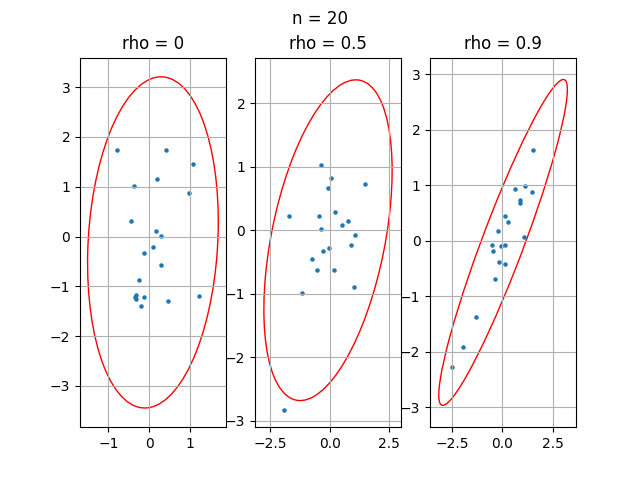
\includegraphics[scale=0.85]{figures/elipse20.png}
        \caption{Эллипс рассеивания для 20 элементов}
    \end{figure}
    
    \begin{figure}[H]
        \centering
        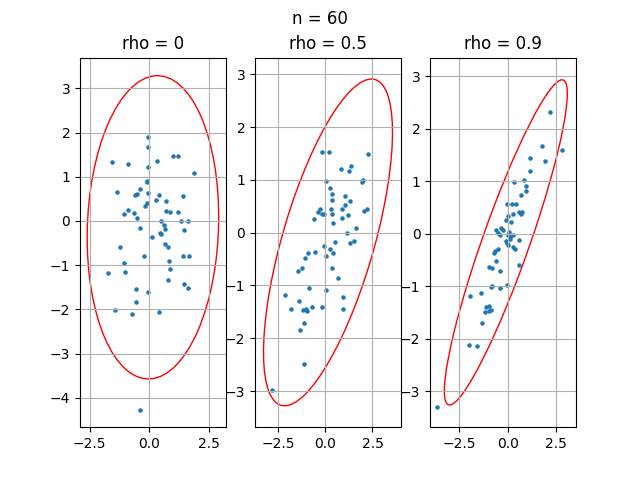
\includegraphics[scale=0.85]{figures/elipse60.png}
        \caption{Эллипс рассеивания для 60 элементов}
    \end{figure}
    
    \begin{figure}[H]
        \centering
        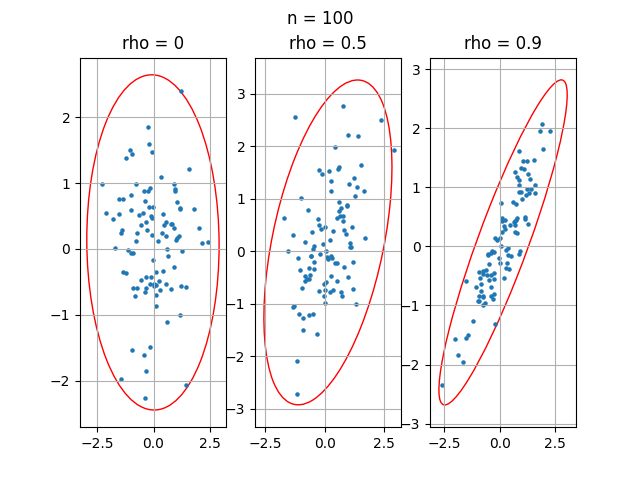
\includegraphics[scale=0.85]{figures/elipse100.png}
        \caption{Эллипс рассеивания для 100 элементов}
    \end{figure}
    
    \subsection{Оценки коэффициентов линейной регрессии}
    \subsubsection{Выборка без возмущений}
		\begin{itemize}
			\item{Критерий наименьших квадратов:}
			$\hat{a}\approx 1.82$, $\hat{b}\approx 2.01$
			\item{Критерий наименьших модулей:}
			$\hat{a}\approx 1.70$, $\hat{b}\approx 1.91$
		\end{itemize}
		\begin{figure}[H]
			\centering
			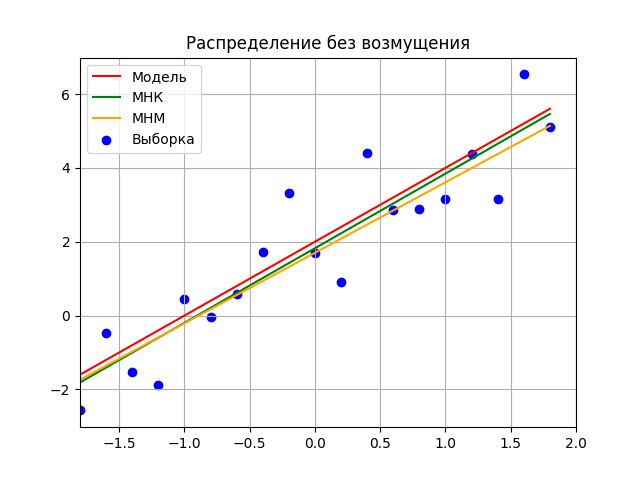
\includegraphics[width = 10cm, height 8cm]{figures/noDisturbance.png}
			\caption{Выборка без возмущений}
			\label{w/o_pert}
		\end{figure}
	
	\subsubsection{Выборка с возмущениями}
		\begin{itemize}
			\item{Критерий наименьших квадратов:}
			$\hat{a}\approx 1.83$, $\hat{b}\approx 0.44$
			\item{Критерий наименьших модулей:}
			$\hat{a}\approx 1.76$, $\hat{b}\approx 1.40$
		\end{itemize}
		\begin{figure}[H]
			\centering
			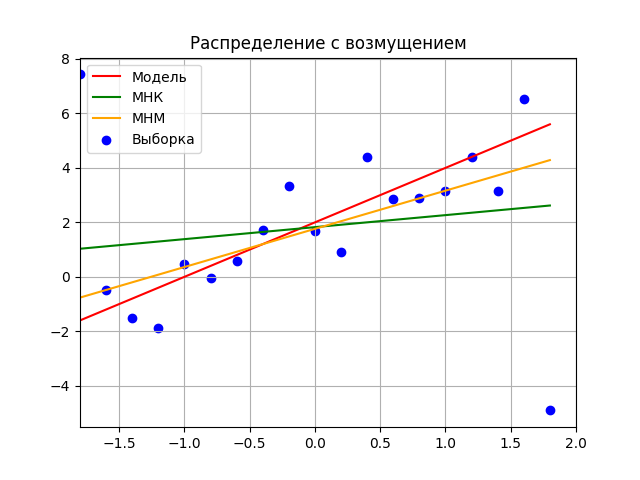
\includegraphics[width = 10cm, height = 8cm]{figures/Disturbance.png}
			\caption{Выборка с возмущениями}
			\label{w_pert}
		\end{figure}
		
		
    \subsection{Проверка гипотезы о законе распределения генеральной совокупности. Метод хи-квадрат}
    
    \noindent Метод максимального правдоподобия:
    \newline
    $\hat{\mu} \approx 0.09, \hat{\sigma} \approx 0.91$
    \newline Критерий согласия $\chi^{2}$:
    \begin{itemize}
        \item Количество промежутков $k = 8$
        \item Уровень значимости $\alpha$= 0.05
        \item Тогда квантиль $\chi^{2}_{1-\alpha}(k-1)$ = $\chi^{2}_{0.95}(7)$. Из таблицы [3, с. 358] $\chi^{2}_{0.95}(7) \approx 14.07$.
    \end{itemize}

    \newline
 
    \begin{table}[H]
    	\centering
    	\begin{tabular}{| c | c | c | c | c | c | c |}
    		\hline
    		$i$ & $limits$         &   $n_i$ &    $p_i$ &   $np_i$ &   $n_i - np_i$ &   $\frac{(n_i-np_i)^2}{np_i}$ \\
    		\hline
                 1 & ['-inf', -1.1]     &   9 & 0.1357 &  13.5666 & -4.5666 & 1.5371 \\
                 2 & [-1.1, -0.7333]    &  11 & 0.096  &   9.6012 &  1.3988 & 0.2038 \\
                 3 & [-0.7333, -0.3667] &   8 & 0.1253 &  12.5256 & -4.5256 & 1.6352 \\
                 4 & [-0.3667, 0.0]     &  15 & 0.1431 &  14.3066 &  0.6934 & 0.0336 \\
                 5 & [0.0, 0.3667]      &  18 & 0.1431 &  14.3066 &  3.6934 & 0.9535 \\
                 6 & [0.3667, 0.7333]   &  17 & 0.1253 &  12.5256 &  4.4744 & 1.5983 \\
                 7 & [0.7333, 1.1]      &   6 & 0.096  &   9.6012 & -3.6012 & 1.3507 \\
                 8 & [1.1, 'inf']       &  16 & 0.1357 &  13.5666 &  2.4334 & 0.4365 \\
                $\sum$ & -              & 100 & 1      & 100      & 0       & 7.7487 \\
    		\hline
    	\end{tabular}
    	\caption{ Вычисление $\chi^{2}_{B}$ при проверке гипотезы $H_{0}$ о нормальном законе распределения $N(x,\hat{\mu}, \hat{\sigma})$}
    	\label{tab:normal_chi_2}
    \end{table} 
    
    \noindent Сравнивая $\chi^{2}_{B} = 7.74$ и $\chi^{2}_{0.95}(7) \approx 14.07$, видим, что $\chi^{2}_{B} < \chi^{2}_{0.95}$.
    \\
    
    \begin{table}[H]
    	\centering
    	\begin{tabular}{| c | c | c | c | c | c | c |}
    		\hline
    		$i$ & $limits$         &   $n_i$ &    $p_i$ &   $np_i$ &   $n_i - np_i$ &   $\frac{(n_i-np_i)^2}{np_i}$ \\
    		\hline
                 1 & ['-inf', -1.1]    &  2 & 0.1357 &  2.7133 & -0.7133 & 0.1875 \\
                 2 & [-1.1, -0.3667]   &  5 & 0.2213 &  4.4254 &  0.5746 & 0.0746 \\
                 3 & [-0.3667, 0.3667] &  7 & 0.2861 &  5.7226 &  1.2774 & 0.2851 \\
                 4 & [0.3667, 1.1]     &  2 & 0.2213 &  4.4254 & -2.4254 & 1.3292 \\
                 5 & [1.1, 'inf']      &  4 & 0.1357 &  2.7133 &  1.2867 & 0.6102 \\
                 $\sum$                & 20 & 1      & 20      &  0      & 2.4867 \\
    		\hline
    	\end{tabular}
    	\caption{ Вычисление $\chi^{2}_{B}$ при проверке гипотезы $H_{0}$ о законе распределения $L(x,\hat{\mu}, \hat{\sigma})$, $n=20$}
    	\label{tab:laplace_chi_2}
    \end{table}
    
    \noindent Сравнивая $\chi^{2}_{B} = 2.48$ и $\chi^{2}_{0.95}(4) \approx 9.49$, видим, что $\chi^{2}_{B} < \chi^{2}_{0.95}$.
    \\
    
    \subsection{Доверительные интервалы для параметров нормального распределения}
	\begin{table}[H]
	    \centering
	    \begin{tabular}{| c | c | c |}
	    \hline
	       n = 20   &  $m$  & $\sigma$\\ \hline
	          &  -0.64 < $m$ < 0.37 & 0.82 < $\sigma$ < 2.0 \\ \hline
	         &   &   \\ \hline
	       n = 100   &  $m$  & $\sigma$\\ \hline
	        & -0.11 < $m$ < 0.29 & 0.89 < $\sigma$ < 1.0 \\
	   \hline
	    \end{tabular}
	    \caption{Доверительные интервалы для параметров нормального распределения}
	    \label{tab:interv_simple}
	\end{table}
	
\subsection{Доверительные интервалы для параметров произвольного распределения. Асимптотический подход}
	\begin{table}[H]
	    \centering
	    \begin{tabular}{| c | c | c |}
	    \hline
	       n = 20   &  $m$  & $\sigma$\\ \hline
	          &  -0.57 < $m$ < 0.31 & 0.87 < $\sigma$ < 1.41 \\ \hline
	         &   &   \\ \hline
	       n = 100   &  $m$  & $\sigma$\\ \hline
	        & -0.11 < $m$ < 0.29 & 0.88 < $\sigma$ < 1.21 \\
	   \hline
	    \end{tabular}
	    \caption{Доверительные интервалы для параметров произвольного распределения. Асимптотический подход}
	    \label{tab:interv_asimpt}
	\end{table}
\end{document}